\documentclass[xcolor={dvipsnames}]{beamer}

\usetheme{metropolis}
\usepackage{calligra}
\usepackage{LobsterTwo}
\usepackage{tikz}
\usepackage{bm}
\usepackage{minted}
\usepackage{graphicx}

\newcommand*\circled[1]{\tikz[baseline=(char.base)]{
            \node[shape=circle, draw, inner sep=0.8pt] (char) {#1};}}
         
         
\title{Relation Extraction \\ \qquad \& \\ Drug Drug Interaction Extraction}
\date{\today}
\author{\LobsterTwo Shi XiuFeng}
\institute{SCHOOL OF SOFTWARE, DALIAN UNIVERSITY OF TECHNOLOGY}

\begin{document}

\maketitle

\section{Relation Extraction}

\begin{frame}{\insertsection}

\begin{alertblock}{General Definition}

{``A relationship extraction task requires the detection and classification of semantic relationship mentions within a set of artifacts, typically from text or XML documents.''}
  \vskip5mm
  \hspace*\fill{--- Wikipedia}

\end{alertblock}

\end{frame}

\begin{frame}{\insertsection}

\begin{alertblock}{Mathematical Definition}

		A relation is defined in the form of a tuple $\bm{t} = (e_1, e_2, \dots, e_n)$ \\
		where the $\bm{e_i}$ are entities in a predefined relation $\bm{r}$ within \\ 
		document $\bm{D}$.

\end{alertblock}

\end{frame}

\begin{frame}{\insertsection}

	\begin{exampleblock}{Types}
		\begin{itemize}
			\item binary relations
			\begin{itemize}
				\item located-in (CMU, Pittsburgh)
				\item father-of (Manuel Blum, Avrim Blum)
				\item etc.
			\end{itemize}
			\item high-order relations
			\begin{itemize}
				\item "At \textcolor{blue}{codons 12}, the occurrence of point mutations from \textcolor{blue}{G} to \textcolor{blue}{T} were observed" $\to$ point-mutation(condon, 12, G, T)
				\item etc.
			\end{itemize}
		\end{itemize}
	\end{exampleblock}
\end{frame}

\begin{frame}{\insertsection}

\begin{exampleblock}{Applications}
		\begin{itemize}
			\item Gene Disease Relationships Extraction
			\item Protein Protein Interaction Extraction
			\item Drug Drug Interaction Extraction
			\item Machine Reading
		\end{itemize}
\end{exampleblock}
\end{frame}

\begin{frame}{\insertsection}

\begin{exampleblock}{Applications}
		\begin{itemize}
			\item Gene Disease Relationships Extraction
			\item Protein Protein Interaction Extraction
			\item \alert{Drug Drug Interaction Extraction}
			\item Machine Reading
		\end{itemize}
\end{exampleblock}
\end{frame}

\begin{frame}[fragile]{\insertsection}
   \makebox[\textwidth][c]{
      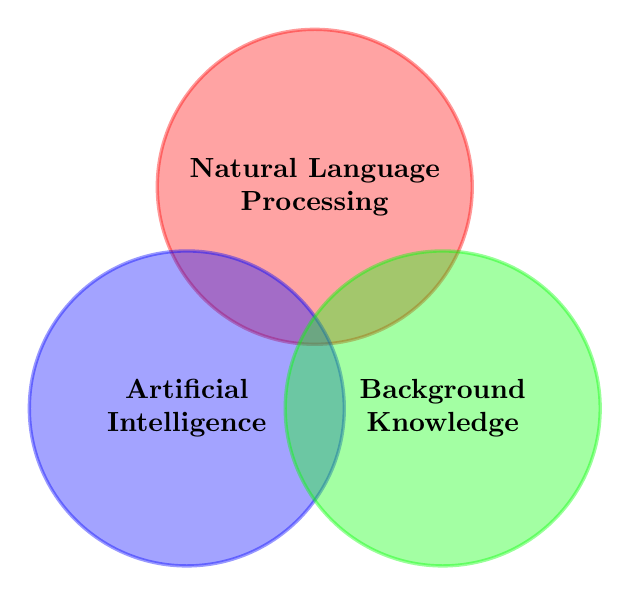
\begin{tikzpicture}[venn circle/.style={draw=#1,
               circle,
               very thick,
               minimum width=4cm,
               text=black,
               fill=#1!90,
               opacity=0.4,
               text opacity=1},
         every node/.append style={align=center}]
         \node [venn circle = red] (A) at (60:3.25cm) {\textbf{Natural Language} \\ \textbf{Processing}};
         \visible<2->{\node [venn circle = blue] (B) at (0,0) {\textbf{Artificial} \\ \textbf{Intelligence}};
         \visible<3->{\node [venn circle = green] (C) at (0:3.25cm) {\textbf{Background} \\ \textbf{Knowledge}};}}
      \end{tikzpicture}
   }
\end{frame}

\begin{frame}{\insertsection}

\begin{exampleblock}{Old School Methods}
		\begin{itemize}
			\item Supervised Methods
				\begin{itemize}
					\item feature based methods
					\item kernel based methods
				\end{itemize}
			\item Semi-supervised and Bootstrapping Methods
				\begin{itemize}
					\item DIPRE
					\item Snowball
					\item KnowItAll
					\item TextRunner
				\end{itemize}
			\end{itemize}
\end{exampleblock}
\end{frame}

\begin{frame}{\insertsection}

\begin{exampleblock}{Deep Learning Methods}
		\begin{itemize}
			\item Deep Neural Networks
			\item Convolutional Neural Networks
			\item Recurrent Neural Networks
				\begin{itemize}
					\item Long Short Term Memory Networks
					\item Bidirectional Long Short Term Memory Networks
					\item Attention-based Models
				\end{itemize}
			\end{itemize}
\end{exampleblock}
\end{frame}

\begin{frame}{\insertsection}

\begin{exampleblock}{Evaluations in SemEval}
		\begin{itemize}
			\small 
			\item SemEval-2007 Task 4 \\ Classification of Semantic Relations between Nominals
			\item SemEval-2010 Task 8 \\ Multi-Way Classification of Semantic Relations Between Pairs of Nominals
			\item SemEval-2013 Task 9 \\ Extraction of Drug-Drug Interactions From BioMedical Texts
			\item SemEval-2017 Task 10 \\ Extracting Key Phrases and Relations From Scientific Publications
			\item SemEval-2018 Task 7 \\ Semantic Relation Extraction and Classification in Scientific Papers
		\end{itemize}
\end{exampleblock}
\end{frame}

\begin{frame}{\insertsection}

\begin{exampleblock}{Evaluations in SemEval}
		\begin{itemize}
			\small 
			\item SemEval-2007 Task 4 \\ Classification of Semantic Relations between Nominals
			\item \alert{SemEval-2010 Task 8 \\ Multi-Way Classification of Semantic Relations Between Pairs of Nominals}
			\item SemEval-2013 Task 9 \\ Extraction of Drug-Drug Interactions From BioMedical Texts
			\item SemEval-2017 Task 10 \\ Extracting Key Phrases and Relations From Scientific Publications
			\item SemEval-2018 Task 7 \\ Semantic Relation Extraction and Classification in Scientific Papers
		\end{itemize}
\end{exampleblock}
\end{frame}

\subsection{Evaluations in SemEval}

\section{Drug Drug Interaction Extraction}

\begin{frame}{\insertsection}

\begin{alertblock}{Task Description}

The goal of the task is to provide a common framework for evaluation of information extraction techniques applied to the \underline{\textbf{\circled{\small{1}}\;recognition}} of pharmacological substances and \underline{\textbf{\circled{\small{2}}\;detection}} of drug-drug interactions from \textit{biomedical texts}.

\end{alertblock}

\end{frame}

\begin{frame}{\insertsection}

\begin{alertblock}{Task Description}

The goal of the task is to provide a common framework for evaluation of information extraction techniques applied to the \underline{\textbf{\circled{\small{1}}\;recognition}} of pharmacological substances and \alert{\underline{\textbf{\circled{\small{2}}\;detection}}} of drug-drug interactions from \textit{biomedical texts}.

\end{alertblock}

\end{frame}

\begin{frame}{\insertsection}

\begin{exampleblock}{Dataset Description}
\begin{itemize}
\item 714 Documents: 
\item 27792 Pairs: 
\item 4 Kinds of DDI Types
    \begin{itemize}
    	\item Advice
		\item Effect
		\item Mechanism
		\item Int
    \end{itemize}
\end{itemize}
\end{exampleblock}
\end{frame}

\begin{frame}[fragile]{\insertsection}
\begin{minted}[fontsize=\scriptsize, linenos]{xml}

<?xml version="1.0" encoding="UTF-8"?>
<document id="DDI-MedLine.d13">
    (...)
    <sentence id="DDI-MedLine.d13.s5" 
              text="On the basis of the estimated number of
                    regular users of intravenous amphetamine in
                    Ontario, the mortality rate in such users is 
                    at least four times as high as in the general 
                    population of the same age, and is comparable 
                    to that in alcoholics and heroin addicts. ">
        <entity id="DDI-MedLine.d13.s7.e0"
                charOffset="69-79" type="drug" text="amphetamine"/>
        <entity id="DDI-MedLine.d13.s7.e1"
                charOffset="247-252" type="drug_n" text="heroin"/>
        <pair id="DDI-MedLine.d13.s7.p0" e1="DDI-MedLine.d13.s7.e0"
              e2="DDI-MedLine.d13.s7.e1" ddi="false"/>
    </sentence>
    (...)
</document>

\end{minted}

\end{frame}

\begin{frame}[fragile]{\insertsection}
\begin{minted}[fontsize=\scriptsize, linenos]{xml}

<?xml version="1.0" encoding="UTF-8"?>
<document id="DDI-MedLine.d13">
    (...)
    <sentence id="DDI-MedLine.d13.s5" 
              text="On the basis of the estimated number of
                    regular users of intravenous amphetamine in
                    Ontario, the mortality rate in such users is 
                    at least four times as high as in the general 
                    population of the same age, and is comparable 
                    to that in alcoholics and heroin addicts. ">
        <entity id="DDI-MedLine.d13.s7.e0"
                charOffset="69-79" type="drug" text="amphetamine"/>
        <entity id="DDI-MedLine.d13.s7.e1"
                charOffset="247-252" type="drug_n" text="heroin"/>
        <pair id="DDI-MedLine.d13.s7.p0" e1="DDI-MedLine.d13.s7.e0"
              e2="DDI-MedLine.d13.s7.e1" ddi="false"/>
    </sentence>
    (...)
</document>

\end{minted}

\end{frame}

\begin{frame}[fragile]{\insertsection}
\begin{minted}[fontsize=\scriptsize, linenos]{xml}

<?xml version="1.0" encoding="UTF-8"?>
<document id="DDI-MedLine.d13">
    (...)
    <sentence id="DDI-MedLine.d13.s5" 
              text="On the basis of the estimated number of
                    regular users of intravenous amphetamine in
                    Ontario, the mortality rate in such users is 
                    at least four times as high as in the general 
                    population of the same age, and is comparable 
                    to that in alcoholics and heroin addicts. ">
        <entity id="DDI-MedLine.d13.s7.e0"
                charOffset="69-79" type="drug" text="amphetamine"/>
        <entity id="DDI-MedLine.d13.s7.e1"
                charOffset="247-252" type="drug_n" text="heroin"/>
        <pair id="DDI-MedLine.d13.s7.p0" e1="DDI-MedLine.d13.s7.e0"
              e2="DDI-MedLine.d13.s7.e1" ddi="false"/>
    </sentence>
    (...)
</document>
\end{minted}

\end{frame}

\begin{frame}[fragile]{\insertsection}

\begin{alertblock}{Methods}

\begin{itemize}
\item S. K. Sahu and A. Anand, \textbf{“Drug-drug interaction extraction from biomedical text using long short term memory network.”} arXiv preprint arXiv:1701.08303, 2017.
\item Z. Zhao, Z. Yang, L. Luo, H. Lin, and J. Wang, \textbf{“Drug drug interaction extraction from biomedical literature using syntax convolutional neural network.”} Bioinformatics, vol. 32, no. 22, pp. 3444–3453, 2016.
\end{itemize}
\end{alertblock}
\end{frame}

\section{Drug-drug interaction extraction from biomedical text using long short term memory network}
\subsection{Drug-drug interaction extraction from biomedical text ...}

\begin{frame}{\insertsubsection}

\begin{exampleblock}{Preprocessing}
\begin{itemize}
\item Tokenization
	\begin{itemize}
		\item Genia Tagger
		\item All digits $\to$ DG
		\item All letters $\to$ lowercase
	\end{itemize}
\item Targeted drug names are replaced with \underline{DRUG-A} and \underline{DRUG-B}, other drug names are replaced with \underline{DRUG-N}.
\end{itemize}
\end{exampleblock}

\end{frame}

\begin{frame}{\insertsubsection}

\begin{exampleblock}{Negative Instance Filtering}
\begin{itemize}
\item Remove instances whose targeted drug names are the same as each other. We assume that a drug doesn't interact with itself.
\item Remove negative samples based on some grammatical patterns:
	\begin{itemize}
		\item DRUG-A (DRUG-B)
		\item DRUG-A such as DRUG-B
		\item DRUG-A $\text{(DRUG-N)}^+$ DRUG-B
		\item etc.
	\end{itemize}
\end{itemize}
\end{exampleblock}

\end{frame}

\begin{frame}{\insertsubsection}

\begin{exampleblock}{Negative Instance Filtering}
\begin{figure}[ht]
\centering
\includegraphics[scale=0.35]{table1.png}
\end{figure}
\end{exampleblock}

\end{frame}

\begin{frame}{\insertsubsection}

\begin{exampleblock}{Presented Models}

\begin{itemize}
\item B-LSTM, B for Bidirectinal
\item AB-LSTM, A for Attentive
\item Joint AB-LSTM
\end{itemize}

\end{exampleblock}

\end{frame}


\begin{frame}{\insertsubsection}

\begin{exampleblock}{B-LSTM}
\begin{figure}[ht]
\centering
\includegraphics[scale=0.255]{fig1.png}
\end{figure}
\end{exampleblock}

\end{frame}


\begin{frame}{\insertsubsection}

\begin{exampleblock}{AB-LSTM}
\begin{figure}[ht]
\centering
\includegraphics[scale=0.27]{fig2.png}
\end{figure}
\end{exampleblock}

\end{frame}

\begin{frame}{\insertsubsection}

\begin{exampleblock}{Joint AB-LSTM}
\begin{figure}[ht]
\centering
\includegraphics[scale=0.195]{fig3.png}
\end{figure}
\end{exampleblock}

\end{frame}

\begin{frame}{\insertsubsection}

\begin{exampleblock}{Performance}
\begin{figure}[ht]
\centering
\includegraphics[scale=0.30]{fig4.png}
\end{figure}
\end{exampleblock}

\end{frame}

\begin{frame}
\begin{center}
\Huge \calligra Fin.
\end{center}
\end{frame}


\end{document}
